

\documentclass{beamer}

\mode<presentation> {

\usetheme{Madrid}

\setbeamertemplate{footline}[page number] % To replace the footer line in all slides with a simple slide count uncomment this line

%\setbeamertemplate{navigation symbols}{} % To remove the navigation symbols from the bottom of all slides uncomment this line
}
\usepackage[utf8]{inputenc}
\usepackage[brazil]{babel}
\usepackage{subfig}
\usepackage{graphicx} % Allows including images
\usepackage{booktabs} % Allows the use of \toprule, \midrule and \bottomrule in tables

%----------------------------------------------------------------------------------------
%	TITLE PAGE
%----------------------------------------------------------------------------------------

\title[ ]{\textbf{Modelo de otimização mutiobjetivo para adequação de embarcações de alta velocidade}\\Apresentação Parcial PAIC 2017/2018} % The short title appears at the bottom of every slide, the full title is only on the title page

\author[L.E.F.B]{Luiz Eduardo Fernandes Bentes, Renata da Encarnação Onety} % Your name
\institute[UEA] % Your institution as it will appear on the bottom of every slide, may be shorthand to save space
{
Universidade do Estado do Amazonas \\ Escola Superior de Tecnologia -- EST\\ Manaus - Amazonas - Brasil\\ % Your institution for the title page
\medskip
\textit{\{lefb.eng,ronety\} @uea.edu.br} % Your email address
}
\date{\today} % Date, can be changed to a custom date

\begin{document}

\begin{frame}
\titlepage % Print the title page as the first slide
\end{frame}

\begin{frame}
\frametitle{Overview}
\tableofcontents
\end{frame}

%------------------------------------------------
\section{Introdução} 
%------------------------------------------------
\begin{frame}
 \tableofcontents[ 
    currentsubsection, 
    hideothersubsections, 
    sectionstyle=show/shaded
    ] 
\end{frame}
%-------------------------------------------------
\begin{frame}
\frametitle{Introdução}
\begin{itemize}
	\item Para prestar socorro à população em atendimentos de urgência e emergência em saúde, as regiões sem acesso terrestre contam com o serviço de SAMU Fluvial.
	\item Atendimento similiar às ambulâncias terrestes.
\end{itemize}

\begin{figure}[h]
	\centering
	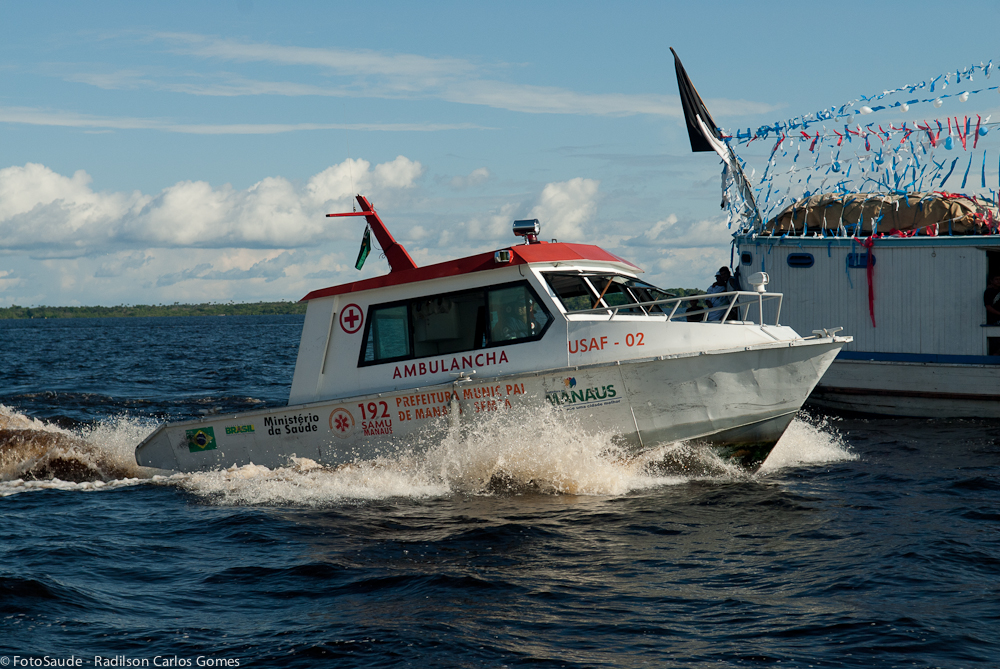
\includegraphics[scale=0.7]{samu17}
	\caption{Ambulâncias Fluviais}
	\label{fig:ambulancha}
\end{figure}

\end{frame}

%------------------------------------------------
\section{Justificativa}
%------------------------------------------------
\begin{frame}
\tableofcontents[ 
    currentsubsection, 
    hideothersubsections, 
    sectionstyle=show/shaded
    ] 
\end{frame}
%-------------------------------------------------
\begin{frame}
\frametitle{Justificativa}
\begin{itemize}
\item Fábrica do Polo Industrial de Manaus
\item Produção de \textbf{70 modelos} de placas diferentes.
\item Máquina NXT 
\end{itemize}


\begin{figure}[h]
\centering
\subfloat[Máquina NXT similar à utilizada na empresa]{
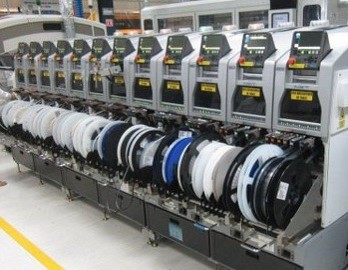
\includegraphics[scale=0.7]{Imagem1}
\label{fig:nxt}
}
\quad 
\subfloat[Carretéis de Componentes]{
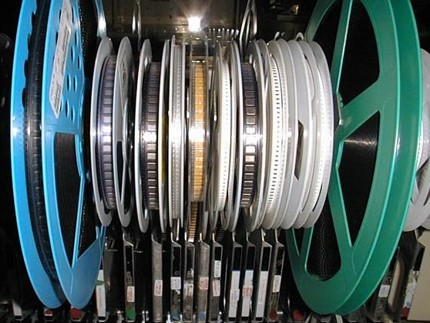
\includegraphics[scale=0.725]{Imagem2}
\label{fig:carreteis}
}
\caption{Máquina NXT e carretéis de componentes}
\end{figure}

\end{frame}

%------------------------------------------------
\begin{frame}
\begin{figure}[h]
\centering
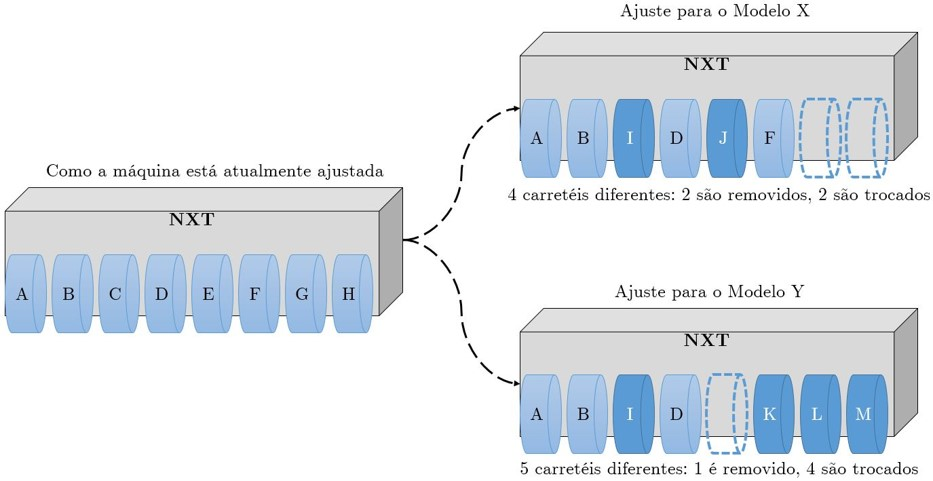
\includegraphics[scale=0.7]{Imagem3}
\caption{Cenário hipotético de escolha de \textit{setup}}
\label{fig:funcionamentoNxt}
\end{figure}
\end{frame}
%------------------------------------------------
\section{Objetivos}
%------------------------------------------------
\begin{frame}
\tableofcontents[ 
    currentsubsection, 
    hideothersubsections, 
    sectionstyle=show/shaded
    ] 
\end{frame}
%-------------------------------------------------
\begin{frame}
\frametitle{Objetivos}
\large
\begin{block}{Objetivo Geral}
Estudar o problema de sequenciamento em uma única máquina com tempos de \textit{setup} dependentes da sequência, minimizando o tempo total para completar o processamento.
\end{block}
\pause
\begin{block}{Objetivos Específicos}
\begin{itemize}
\item Coletar dados referentes ao número de modelos de placas produzidas, os insumos utilizados e aos atuais tempos de \textit{setup};
\item Implementar dois métodos, sendo um de otimização baseado em programação dinâmica, e outro da regra de menor tempo de \textit{setup} em algoritmo guloso;
\item Testar os métodos utilizando os dados coletados e instâncias clássicas da literatura, cujas soluções ótimas são conhecidas.
\item Comparar o desempenho entre os dois métodos.
\end{itemize}

\end{block}

\end{frame}


%------------------------------------------------
\section{Fundamentação Teórica}
%------------------------------------------------
\begin{frame}
\tableofcontents[ 
    currentsubsection, 
    hideothersubsections, 
    sectionstyle=show/shaded
    ] 
\end{frame}
%-------------------------------------------------
	\subsection{Problemas de Sequenciamento}
\begin{frame}
\frametitle{Problemas de Sequenciamento}
\begin{block}{Scheduling}
“Um processo de decisão utilizado regularmente em muitas indústrias de manufatura e de serviços, que lida com a alocação de recursos para tarefas através de dados períodos de tempo e seu objetivo é otimizar um ou mais critérios” \cite{pinedo2015scheduling}. 
\end{block}

\begin{block}{Notação de Graham}
Identificar os problemas de \textit{scheduling} de forma individual
\end{block}

\end{frame}    

%------------------------------------------------
\subsection{Problema Máquina Única}
\begin{frame}{Problema $1|s_{jk}|C_{max}$}
\begin{itemize}
\item De forma simplificada o problema de sequenciamento neste cenário é: 
\begin{equation}
1|s_{jk}|C_{max}
\end{equation}
\item Entretantro no cotidiano da empresa, a situação é mais complexa: 
\begin{equation}
1|s_{jk}, r_{j},d_{j},prmp,prec|C_{max}
\end{equation}



\item O \textit{Makespan} é definido, matematicamente, por: 
\begin{equation}
C_{max} = \sum_{j=1}^{n}p[j] + \sum_{j=1}^{n}s[j-1],[j]
\end{equation}

\end{itemize}
\end{frame}
%------------------------------------------------
\subsection{Similaridades com o Problema do Caixeiro Viajante}
\begin{frame}{Similaridades com o Problema do Caixeiro Viajante}
\begin{block}{Definição}
\begin{center}
``Um vendedor precisa passar por várias cidades afim de vender seus produtos e precisa descobrir o menor percurso entre estas cidades, passando apenas uma vez por cada uma e retornar para a cidade inicial, economizando tempo e custos de transporte''.\\

\textbf{Qual seria a melhor rota a ser escolhida?}
\end{center}
\end{block}
\begin{figure}[h]
\centering
\subfloat[Representação das cidades a serem visitadas]{
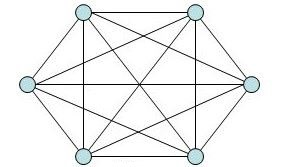
\includegraphics[scale=0.5]{Imagem5}
\label{fig:grafo}
}
\quad 
\subfloat[Esquema exemplificando o tempo de setup entre modelos]{
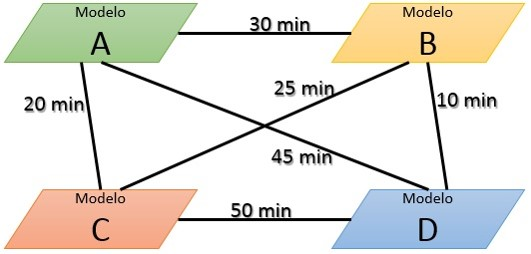
\includegraphics[scale=0.5]{Imagem6}
\label{fig:grafoPlacas}
}
\caption{Comparação do Problema $1|s_{jk}|C_{max}$ com o Caixeiro Viajante}
\label{fig01}
\end{figure}
\end{frame}

%------------------------------------------------
\section{Resultados Parciais}
%------------------------------------------------
\begin{frame}
\tableofcontents[ 
    currentsubsection, 
    hideothersubsections, 
    sectionstyle=show/shaded
    ] 
\end{frame}
%-------------------------------------------------
\subsection{Métodos Implementados}
\begin{frame}{Métodos Implementados}
\Large
\begin{itemize}
\item Algoritmo Guloso
\begin{itemize}
\large
\item Regra de Liberação de menor tempo de \textit{setup}.\cite{pacheco2001adoccao} 
\end{itemize}
\bigskip
\item Programação Dinâmica
\begin{itemize}
\large
\item Recursão com apoio de tabela 
\end{itemize}
\end{itemize}

\end{frame}
%-----------------------------------------------
\subsection{Resultados}
\begin{frame}{Resultados}
Regra MST(Algoritmo Guloso):
\begin{table}[h]
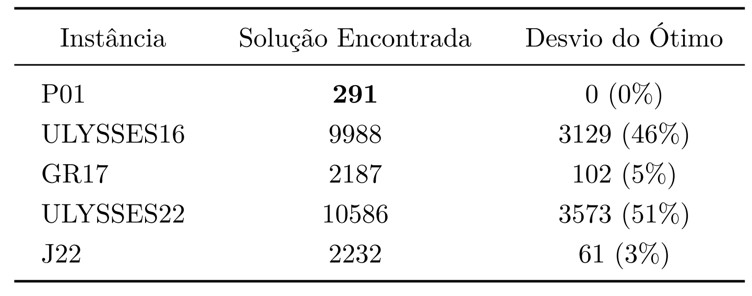
\includegraphics[scale=0.6]{Tabela1}
\end{table}
Otimização por PD:
\begin{table}[h]
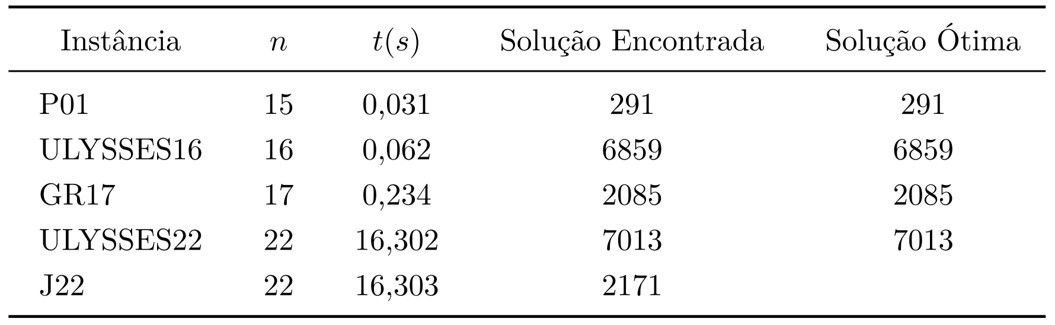
\includegraphics[scale=0.5]{Tabela2}
\end{table}
\end{frame}

%----------------------------------------------
\begin{frame}{Resultados -- Instância P01 }
$n = 15$
\begin{figure}[h]
\centering
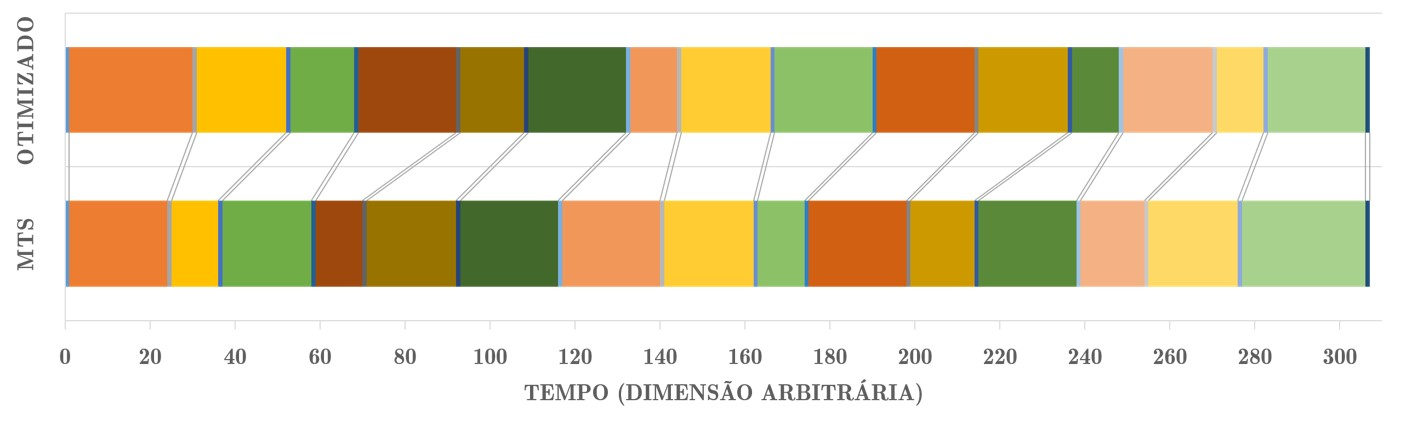
\includegraphics[scale=0.5]{GraficoP01}
\end{figure}
\end{frame}
%---------------------------------------------
\begin{frame}{Resultados -- Instância Ulysses16}
$n = 16$
\begin{figure}[h]
\centering
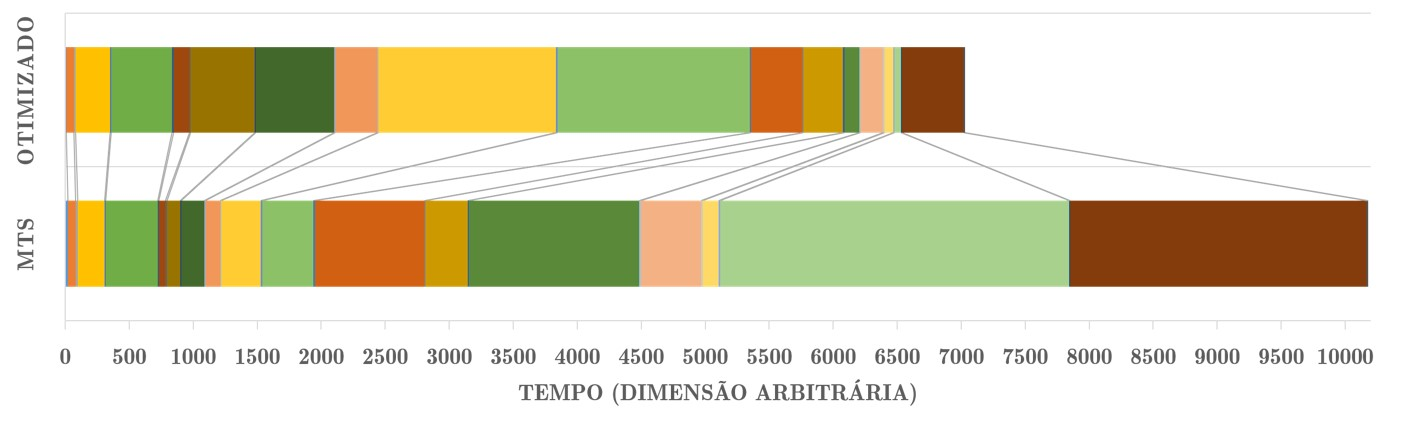
\includegraphics[scale=0.5]{GraficoU16}
\end{figure}
\end{frame}
%----------------------------------------------
\begin{frame}{Resultados -- Instância GR17 }
$n = 17$
\begin{figure}[h]
\centering
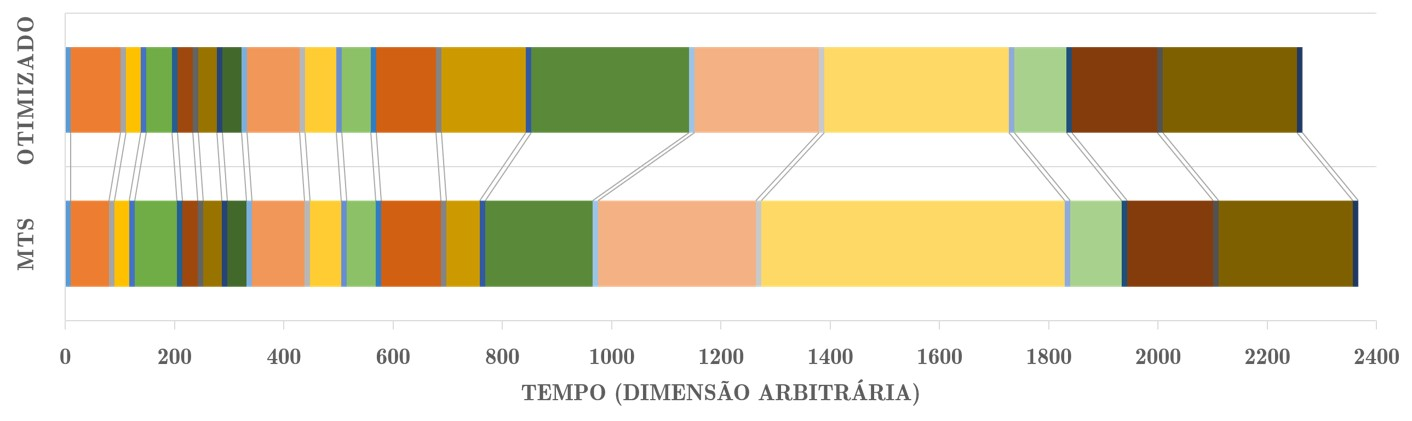
\includegraphics[scale=0.5]{GraficoGR17}
\end{figure}
\end{frame}
%----------------------------------------------
\begin{frame}{Resultados -- Instância J22 }
$n = 22$
\begin{figure}[h]
\centering
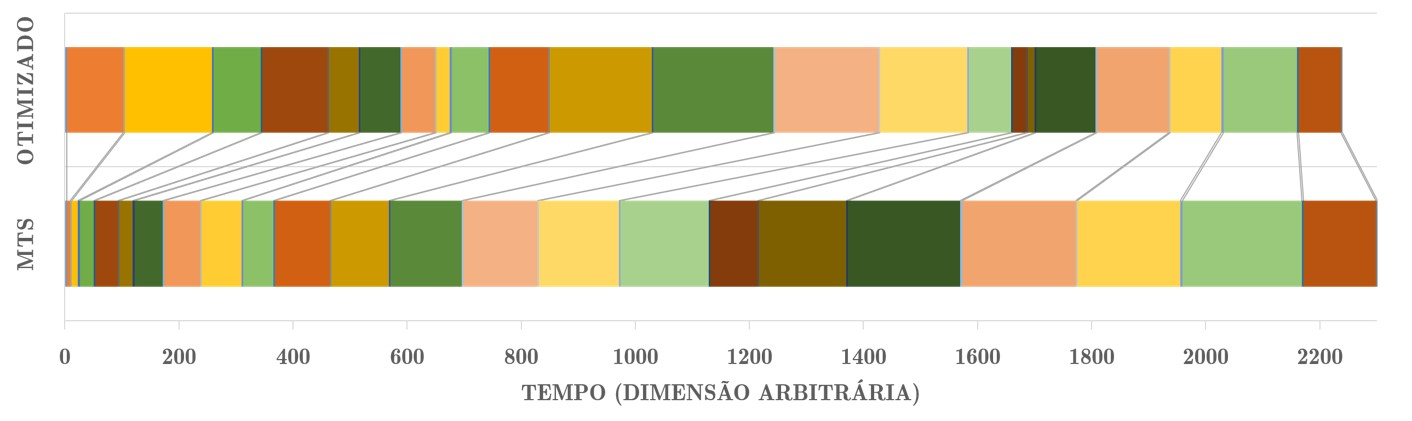
\includegraphics[scale=0.5]{GraficoJ22}
\end{figure}
\end{frame}
%----------------------------------------------
\section{Trabalhos Futuros}
%----------------------------------------------
\begin{frame}
\tableofcontents[ 
    currentsubsection, 
    hideothersubsections, 
    sectionstyle=show/shaded
    ] 
\end{frame}
%-------------------------------------------------
\begin{frame}{Trabalhos Futuros}
\begin{block}{}
\Large
Implementação de Algoritmos Heurísticos para ampliação do tamanho da instância.
\end{block}
\pause
\begin{block}{}
\Large
Desenvolvimento de outras restrições do problema geral:
$1|s_{jk}, r_{j},d_{j},prmp,prec|C_{max}$
\end{block}
\end{frame}

%----------------------------------------------
\section{Cronograma}
%---------------------------------------------
\begin{frame}{Cronograma}
\begin{table}[ht]
\centering

%\caption{My caption}
\label{my-label}
\begin{tabular}{|l|l|}
\hline
\multicolumn{1}{|c|}{Mês} & \multicolumn{1}{c|}{Atividades}                                                                                                                                                    \\ \hline
Março                     & \begin{tabular}[c]{@{}l@{}}Implementação do Algoritmo Genético\\ Desenvolvimento do Artigo para CSBC\\ Estudar Operadores Genéticos\end{tabular}                                   \\ \hline
Abril                     & \begin{tabular}[c]{@{}l@{}}Implementar novos Operadores\\ Desenvolver Componentes Híbridos\\ Implementação de novas restrições do problema geral \textit{Scheduling}\end{tabular} \\ \hline
Maio                      & \begin{tabular}[c]{@{}l@{}}Desenvolvimento do Artigo para SBPO\\ Execução de Testes com instâncias maiores\\ Teste das novas restrições\end{tabular}                               \\ \hline
Junho                     & \begin{tabular}[c]{@{}l@{}}Aperfeiçoar AG\\ Teste de novas instâncias\end{tabular}                                                                                                 \\ \hline
Julho                     & Apresentação Final                                                                                                                                                                 \\ \hline
\end{tabular}
\end{table}
\end{frame}

\section{Referencial Bibliográfico}
%----------------------------------------------
\begin{frame}{Referencial Bibliográfico}
  % estilo da bibliografia
  \bibliographystyle{abbrv}
  % chamando o arquivo refs.bib
  \bibliography{ref}
\end{frame}
% \subsection{Algoritmo Genético}
% \begin{frame}{Algoritmo Genético}

% \begin{itemize}
% \Large
% \item Método Heurístico
% \item Neo-Darwinismo (Evolução das Espécies)
% \item Componentes:
% \begin{itemize}
% \large
% \item Indivíduos
% \item População
% \end{itemize}
% \end{itemize}


% \end{frame}
%---------------------------------------------
% \begin{frame}{Funcionamento - Algoritmo Genético}
% \begin{figure}[h]
% \centering
% 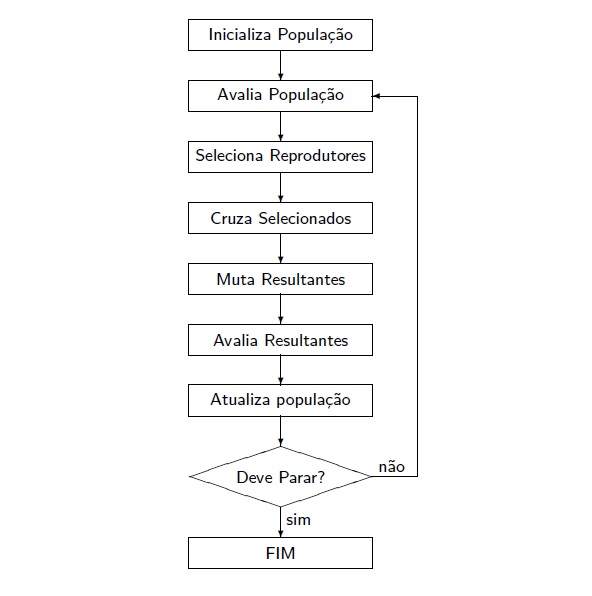
\includegraphics[scale=0.46]{Imagem7}
% \label{fig:funciomanentoAG}
% \caption{Funcionamento do Algoritmo Genético}
% \end{figure}
% \end{frame}
%---------------------------------------------
\begin{frame}
\titlepage
\end{frame}
%---------------------------------------------
\end{document}